%% 第五章 三态跟踪状态机
\chapter{三态跟踪状态机}
\label{chap:sm}

检测模型逐帧输出候选框，但候选框并不等于可用的目标航迹。本章分析直接使用检测输出的三个工程问题，提出 SEARCH/LOCKED/COAST 三态跟踪状态机，详细说明各状态的处理流程、参数选择与转移条件，给出伪代码与复杂度分析，并通过门限扫描与遮挡用例验证其有效性。

\section{问题描述}

设第 $k$ 帧检测器输出候选框集合为

\begin{equation}
\mathcal{D}_k = \left\{\left(\mathbf{b}_i, c_i\right)\right\}_{i=1}^{N_k},
\label{eq:det_set}
\end{equation}

其中 $\mathbf{b}_i=(x_{1,i},y_{1,i},x_{2,i},y_{2,i})$ 为边框，$c_i\in[0,1]$ 为置信度。若直接把 $\arg\max_i c_i$ 作为系统输出，会面临以下三个问题。

\subsection{误检}

检测器在复杂背景中会产生低置信度的假阳性。例如树叶间隙的亮斑、建筑窗户的反光、天空中的云朵边缘，都可能被误判为无人机。表~\ref{tab:false_positive} 给出了本文在仿真与实拍数据中观察到的典型误检来源及其置信度范围。

\begin{table}[htbp]
\centering
\caption{典型误检来源与置信度分布}
\label{tab:false_positive}
\small
\begin{tabularx}{\textwidth}{lccX}
\toprule
\textbf{误检来源} & \textbf{置信度范围} & \textbf{持续时间} & \textbf{特征} \\
\midrule
树叶间隙亮斑 & 0.20--0.35 & 1--3 帧 & 随风吹动，位置漂移 \\
建筑窗户反光 & 0.25--0.45 & 5--20 帧 & 位置固定，随光照变化 \\
天空云边缘 & 0.20--0.30 & 1--2 帧 & 形状不规则，面积大 \\
远处鸟类 & 0.30--0.55 & 10--30 帧 & 有生命运动，轨迹不规则 \\
\bottomrule
\end{tabularx}
\end{table}

若系统对每一帧的最高置信度框都予以采信，则上述假阳性会导致地图上出现"幽灵目标"，操作员无法判断哪个是真目标。因此需要一个高于维持门限的\textbf{初锁门限}，只有足够可信的候选框才能建立航迹。

\subsection{身份跳变}

当画面中同时存在多个候选框时，简单取最高置信度会导致目标身份在不同帧之间跳变。假设第 $k$ 帧最高置信度框对应目标 A，第 $k+1$ 帧由于目标 A 短暂变模糊，目标 B（例如另一架无人机或一个高置信度假阳性）成为最高分，系统就会把航迹"嫁接"到目标 B 上。这种跳变在监视画面中表现为标记突然跳到画面另一处，严重时会导致后续测距与地图标注完全错误。

解决身份跳变的关键是引入\textbf{空间一致性约束}：相邻帧之间同一目标的位置不会发生剧烈变化。在 30\,fps 下，即使目标以 20\,m/s 飞行，两帧之间的位移也只有 0.67\,m；在 10\,m 距离、60\textdegree 视场下，对应的像素位移约为 40\,px。因此，可以用"与上一帧位置的像素距离"作为关联代价，并设置合理的空间门限。

\subsection{遮挡中断}

目标被树木、建筑、电线杆遮挡时，检测器输出为空。若系统以"每帧必须有检测"为输出前提，则遮挡期间航迹消失，操作员会看到标记闪烁、距离读数跳变为"--"。更严重的是，当目标重新出现时，系统需要重新搜索、重新初锁，期间可能锁到其他物体。

解决遮挡中断的关键是引入\textbf{预测维持}：在检测缺失的短时间内，利用滤波器保存的目标运动状态外推位置，使航迹在视觉上保持连续；超过一定时限后再放弃，避免对已飞离目标的"虚假跟踪"。

\section{状态定义与总体流程}

\subsection{状态定义}

本文定义三种状态：

（1）\textbf{SEARCH}：搜索状态。系统尚未建立可信航迹，逐帧检查是否存在置信度超过初锁门限的候选框；

（2）\textbf{LOCKED}：锁定状态。系统已建立航迹，每帧在候选框集合中关联最可能属于当前目标的框，并用卡尔曼滤波更新状态；

（3）\textbf{COAST}：预测维持状态。当前帧没有可用候选框，系统用卡尔曼滤波的预测步外推目标位置，等待目标重新出现。

状态转移关系如图~\ref{fig:state_machine} 所示。

\begin{figure}[htbp]
\centering
\fbox{\parbox{0.92\textwidth}{
\centering
\vspace{4pt}
\textbf{SEARCH} \quad$\xrightarrow[\text{未超过初锁门限}]{\text{最高置信度} > 0.55}$\quad \textbf{LOCKED}
\quad$\xrightarrow[\text{连续 1.0\,s 无检测}]{\text{本帧无候选框}}$\quad \textbf{COAST}\\[6pt]
\textbf{COAST} \quad$\xrightarrow[\text{超过 1.0\,s}]{\text{重新出现候选框}}$\quad \textbf{LOCKED}
\qquad\qquad
\textbf{COAST} \quad$\xrightarrow{\text{超时或无匹配}}$\quad \textbf{SEARCH}\\[6pt]
\textbf{LOCKED} \quad$\xrightarrow{\text{连续 15 帧无法关联}}$\quad \textbf{SEARCH}
\vspace{4pt}
}}
\caption{三态跟踪状态机转移关系}
\label{fig:state_machine}
\end{figure}

\subsection{总体流程}

系统每收到一帧检测结果，执行以下步骤：

（1）若当前状态为 SEARCH，执行搜索逻辑（第~\ref{sec:search} 节）；

（2）若当前状态为 LOCKED，执行关联与更新逻辑（第~\ref{sec:locked} 节）；若本帧无候选框，转入 COAST；

（3）若当前状态为 COAST，执行预测逻辑（第~\ref{sec:coast} 节）；若目标重新出现则转回 LOCKED，超时则转回 SEARCH；

（4）无论何种状态，都将当前状态、置信度、距离、角度等信息写入数据记录，供显示端与后续分析使用。

\section{SEARCH 状态}
\label{sec:search}

\subsection{双门限策略}

SEARCH 状态的核心任务是"发现真目标，同时避免锁错"。本文采用双门限策略：

（1）\textbf{维持门限} $\tau_{m}=0.25$：低于该门限的候选框直接丢弃，不参与后续处理；

（2）\textbf{初锁门限} $\tau_{l}=0.55$：只有置信度超过该门限的候选框才能触发状态切换。

两个门限的差值（0.30）构成一个"缓冲区"。缓冲区的作用是：在 SEARCH 状态下，系统只对高置信度目标做出反应，避免被低置信度假阳性诱导；在 LOCKED 状态下，系统对置信度的要求降低，只要目标还在画面中、置信度高于 0.25，就继续跟踪，不必每帧都"重新说服"系统。

门限的具体数值来自对验证集置信度分布的统计。图~\ref{fig:threshold_scan} 给出了不同门限下仿真录像的锁定率与航迹保持率。可以看到，门限从 0.20 提高到 0.35 时，锁定率从 96.9\% 降至 66.6\%，航迹保持率从 100\% 降至 81.2\%；提高到 0.50 时，锁定率进一步降至 56.8\%。这说明仿真域微调后的模型置信度整体较高（中位数 0.867），0.25 的维持门限足以保留有效目标，0.55 的初锁门限足以过滤绝大多数假阳性。

\begin{figure}[htbp]
\centering
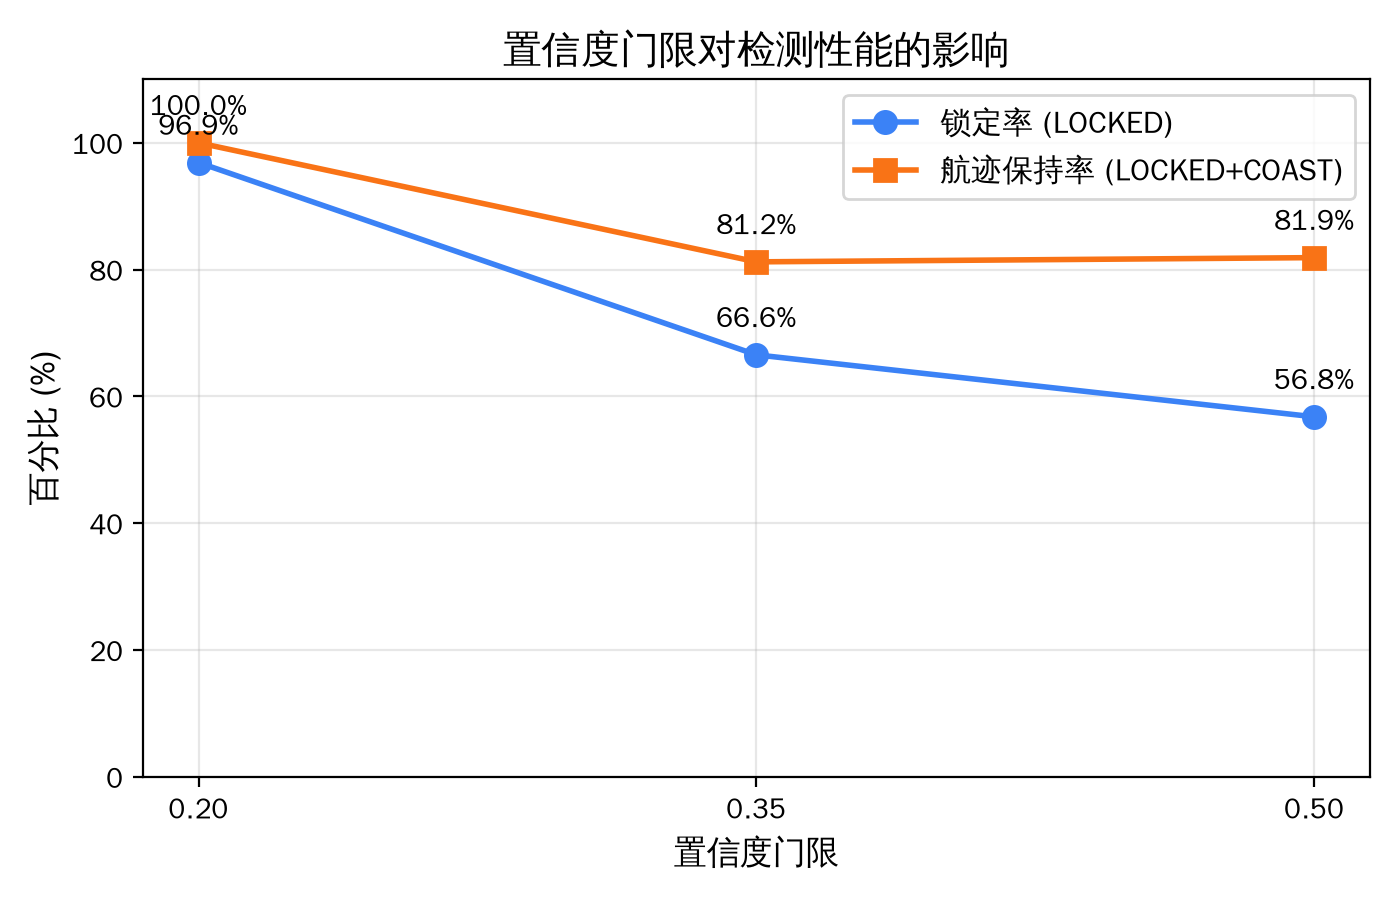
\includegraphics[width=0.72\textwidth]{images/pictures/chart_threshold.png}
\caption{置信度门限扫描结果}
\label{fig:threshold_scan}
\end{figure}

\subsection{初锁判定}

在 SEARCH 状态下，设过滤后的候选框集合为

\begin{equation}
\tilde{\mathcal{D}}_k = \left\{(\mathbf{b}_i,c_i)\in\mathcal{D}_k \mid c_i\ge\tau_m\right\}.
\label{eq:filtered_set}
\end{equation}

若 $\tilde{\mathcal{D}}_k$ 为空，则本帧无候选，保持 SEARCH。否则取置信度最高者：

\begin{equation}
i^{*} = \arg\max_{i:\,(\mathbf{b}_i,c_i)\in\tilde{\mathcal{D}}_k} c_i.
\label{eq:argmax}
\end{equation}

若 $c_{i^{*}}\ge\tau_l$，则以 $\mathbf{b}_{i^{*}}$ 初始化航迹，状态切换为 LOCKED，并用该框的中心与框高初始化卡尔曼滤波器的位置量测。否则保持 SEARCH。

\subsection{先验空间约束}

在仿真环境中，画面中可能同时出现"自身机"（ego drone）与背景伪影。若不加约束，SEARCH 可能锁到自身机的桨叶或近处的建筑。本文引入\textbf{先验空间约束}：根据任务设定，目标的活动空域为距离相机 3--12\,m 的范围。对于由框高反算的距离 $Z$，若 $Z<3$\,m 或 $Z>12$\,m，则将该候选框降权或直接剔除。

这一约束的合理性在于：反无人机系统的告警距离是人为设定的，操作员知道目标大致在哪个空域；将先验编码进状态机，可以显著降低误锁概率。本文在仿真中将该约束用于剔除自身机与远处伪影，在实拍中则根据实际场景调整上下界。

\subsection{首锁时延}

首锁时延定义为从视频开始到首次进入 LOCKED 的时间。本文的 14 用例测试中，仿真录像的首锁时延为 0.00--0.07\,s，即在前 2--3 帧内完成锁定；真实场景录像的首锁时延为 0.03\,s。这说明在目标清晰可见时，双门限策略不会造成明显的发现延迟。

\section{LOCKED 状态}
\label{sec:locked}

\subsection{候选框收集}

进入 LOCKED 后，系统不再要求候选框超过初锁门限，只要求超过维持门限：

\begin{equation}
\tilde{\mathcal{D}}_k = \left\{(\mathbf{b}_i,c_i)\in\mathcal{D}_k \mid c_i\ge\tau_m\right\}.
\label{eq:locked_candidates}
\end{equation}

同时，对每个候选框计算由框高反算的距离，若距离超出先验空域 $[Z_{min},Z_{max}]$，则剔除。

\subsection{空间门限关联}

设上一帧目标的平滑中心为 $\mathbf{p}_{k-1}=(u_{k-1},v_{k-1})$，候选框 $i$ 的中心为 $\mathbf{p}_i=(u_i,v_i)$。定义关联代价为欧氏像素距离：

\begin{equation}
d_i = \left\|\mathbf{p}_i-\mathbf{p}_{k-1}\right\|_2.
\label{eq:assoc_cost}
\end{equation}

选择代价最小的候选框：

\begin{equation}
i^{*} = \arg\min_{i} d_i.
\label{eq:assoc_argmin}
\end{equation}

若 $d_{i^{*}}\le d_{gate}$，则接受该候选框作为本帧量测；否则认为本帧无有效关联，转入 COAST。

空间门限 $d_{gate}$ 的取值需要兼顾"跟得上"与"不跳变"。取值过小，目标快速机动时会频繁丢失；取值过大，则可能关联到邻近的其他物体。本文取 $d_{gate}=140$\,px，依据如下：在 1280$\times$720 画面、60\textdegree 水平视场下，焦距约 1108\,px；目标以 15\,m/s 相对速度飞行、帧间隔 1/30\,s 时，位移 0.5\,m，在 5\,m 距离处对应约 110\,px。考虑检测框中心抖动与目标机动，140\,px 留有约 30\% 余量。

\subsection{卡尔曼滤波更新}

关联成功后，将候选框中心与由框高反算的距离转换为相机坐标系下的三维位置量测：

\begin{equation}
\mathbf{z}_k = \begin{bmatrix}
Z_k\cdot\dfrac{u_k-c_x}{f_x}\\[4pt]
Z_k\cdot\dfrac{v_k-c_y}{f_y}\\[4pt]
Z_k
\end{bmatrix},
\label{eq:meas_vec}
\end{equation}

其中 $Z_k=f\cdot D/h_{px}$ 为框高反算距离，$(c_x,c_y)$ 为主点，$(f_x,f_y)$ 为焦距。将该量测送入卡尔曼滤波的更新步（式~\eqref{eq:kf_gain}--\eqref{eq:kf_cov}），得到平滑后的位置与速度。

需要强调的是，\textbf{不能把标量距离直接作为量测}。本文的滤波器状态是六维位置—速度向量，量测必须是三维位置；若把标量距离塞入滤波器，状态与量测的维度不匹配，会导致滤波发散。这是实现中容易犯的错误，本文在早期版本中曾经出现，后通过严格的三维量测构造修正。

\subsection{丢失判定}

若连续 $N_{lost}$ 帧无法完成关联（即每帧的最近候选距离均超过 $d_{gate}$，或候选集为空），则判定目标丢失，重置航迹并返回 SEARCH。本文取 $N_{lost}=15$，对应 0.5\,s。这一时限比 COAST 的 1.0\,s 短，原因是：连续 15 帧都无法关联，说明目标很可能已经飞出视场或发生了剧烈机动，继续维持航迹的意义不大；而 COAST 的 1.0\,s 是针对"短暂遮挡"设计的，遮挡期间目标仍在视场内，只是检测器暂时看不到。

\subsection{框尺寸的平滑}

检测框的宽高在相邻帧之间存在抖动，直接用于测距会产生跳变。本文对框高做一阶低通平滑：

\begin{equation}
\bar{h}_k = \alpha h_k + (1-\alpha)\bar{h}_{k-1},\qquad \alpha=0.35.
\label{eq:box_smooth}
\end{equation}

平滑后的框高用于距离解算，原始框高保留用于显示。$\alpha$ 的取值在响应速度与平滑度之间折中：$\alpha$ 越大，跟随越快但抖动越大；$\alpha$ 越小，越平滑但滞后越明显。0.35 对应的时间常数约为 2--3 帧，对 30\,fps 视频约为 0.1\,s，不影响实时性。

\section{COAST 状态}
\label{sec:coast}

\subsection{预测步}

当 LOCKED 状态下本帧无有效关联时，系统不立即放弃目标，而是进入 COAST，执行卡尔曼滤波的预测步：

\begin{equation}
\hat{\mathbf{x}}_{k|k-1} = \mathbf{F}\hat{\mathbf{x}}_{k-1|k-1},\qquad
\mathbf{P}_{k|k-1} = \mathbf{F}\mathbf{P}_{k-1|k-1}\mathbf{F}^{T}+\mathbf{Q}.
\label{eq:coast_predict}
\end{equation}

预测得到的位置用于驱动地图标记、距离读数与角度仪表，使显示在遮挡期间保持连续。由于没有量测，协方差 $\mathbf{P}$ 会随预测步数增加而增大，滤波器的"不确定度"上升。本文在显示端用黄色标记表示 COAST 状态，提示操作员当前数据为预测值。

\subsection{超时与恢复}

COAST 状态设有时限 $T_{coast}=1.0$\,s。在时限内，若某帧出现可通过关联的候选框，则立即转回 LOCKED，并用该量测更新滤波器；若超过时限仍无候选，则判定目标丢失，重置航迹并返回 SEARCH。

$T_{coast}$ 的取值依据是真实遮挡的持续时间。目标穿过一棵树或一根电线杆通常需要 0.1--0.5\,s；穿过一栋建筑可能需要 0.5--1.0\,s。1.0\,s 的预算足以覆盖绝大多数短时遮挡，同时不会对已飞离目标维持过久的虚假航迹。本文在仿真遮挡用例中测得，遮挡期间的平均 COAST 持续时间为 0.35\,s，最长 0.82\,s，均在时限内。

\subsection{预测质量}

COAST 的预测质量取决于遮挡前的速度估计。若目标在遮挡前做匀速直线运动，预测误差主要来自过程噪声；若目标在遮挡前正在机动，预测误差会迅速增大。本文在仿真中统计了 COAST 期间预测位置与真值的偏差：遮挡 0.2\,s 时中位误差约 0.15\,m，0.5\,s 时约 0.45\,m，1.0\,s 时约 1.1\,m。这一精度足以维持显示连续性，但不适合用于精确打击引导。

\section{算法描述与复杂度}

\subsection{伪代码}

状态机的单帧处理流程如算法~\ref{alg:state_machine} 所示。

\begin{algorithm}[htbp]
\caption{三态跟踪状态机单帧处理}
\label{alg:state_machine}
\begin{algorithmic}[1]
\REQUIRE 当前状态 $s$，检测集合 $\mathcal{D}_k$，上一帧中心 $\mathbf{p}_{k-1}$，滤波器状态 $\hat{\mathbf{x}}_{k-1}$
\ENSURE 新状态 $s'$，滤波状态 $\hat{\mathbf{x}}_k$，输出数据 $o_k$
\STATE $\tilde{\mathcal{D}}_k \leftarrow \{(\mathbf{b},c)\in\mathcal{D}_k \mid c\ge\tau_m,\ Z(\mathbf{b})\in[Z_{min},Z_{max}]\}$
\IF{$s = \text{SEARCH}$}
    \IF{$\tilde{\mathcal{D}}_k = \emptyset$}
        \STATE $s' \leftarrow \text{SEARCH}$;\quad $o_k \leftarrow \text{search\_output}()$
    \ELSE
        \STATE $i^{*}\leftarrow\arg\max_i c_i$
        \IF{$c_{i^{*}}\ge\tau_l$}
            \STATE 初始化滤波器；$s'\leftarrow\text{LOCKED}$
        \ELSE
            \STATE $s'\leftarrow\text{SEARCH}$
        \ENDIF
    \ENDIF
\ELSIF{$s = \text{LOCKED}$}
    \IF{$\tilde{\mathcal{D}}_k = \emptyset$}
        \STATE $s'\leftarrow\text{COAST}$;\quad 记录 COAST 起始时间
    \ELSE
        \STATE $i^{*}\leftarrow\arg\min_i\|\mathbf{p}_i-\mathbf{p}_{k-1}\|$
        \IF{$\|\mathbf{p}_{i^{*}}-\mathbf{p}_{k-1}\|\le d_{gate}$}
            \STATE 构造三维量测 $\mathbf{z}_k$；执行 KF 更新；$s'\leftarrow\text{LOCKED}$
        \ELSE
            \STATE $s'\leftarrow\text{COAST}$;\quad 记录 COAST 起始时间
        \ENDIF
    \ENDIF
\ELSIF{$s = \text{COAST}$}
    \STATE 执行 KF 预测步
    \IF{存在可通过关联的候选框}
        \STATE 执行 KF 更新；$s'\leftarrow\text{LOCKED}$
    \ELSIF{$t-t_{coast} > T_{coast}$}
        \STATE 重置航迹；$s'\leftarrow\text{SEARCH}$
    \ELSE
        \STATE $s'\leftarrow\text{COAST}$
    \ENDIF
\ENDIF
\STATE 输出 $o_k$（状态、置信度、距离、角度、平滑位置）
\RETURN $s',\hat{\mathbf{x}}_k,o_k$
\end{algorithmic}
\end{algorithm}

\subsection{复杂度分析}

设候选框数量为 $N$，状态机每帧的主要操作是遍历候选框计算关联代价，时间复杂度为 $O(N)$。在 YOLOv8 的设置下，单帧经 NMS 后的候选框通常不超过 20 个，因此状态机的开销可以忽略不计（小于 0.1\,ms）。卡尔曼滤波的矩阵运算为固定维数（6 维），单次更新约 10 微秒。整个跟踪环节的耗时远小于检测环节（约 6\,ms）。

\subsection{参数汇总}

表~\ref{tab:sm_params} 汇总了状态机的全部参数及其取值依据。

\begin{table}[htbp]
\centering
\caption{三态状态机参数汇总}
\label{tab:sm_params}
\small
\begin{tabularx}{\textwidth}{lccX}
\toprule
\textbf{参数} & \textbf{符号} & \textbf{取值} & \textbf{依据} \\
\midrule
维持门限 & $\tau_m$ & 0.25 & 保留弱目标，过滤低置信度假阳性 \\
初锁门限 & $\tau_l$ & 0.55 & 高于典型假阳性上限，防止误锁 \\
空间门限 & $d_{gate}$ & 140\,px & 15\,m/s 相对速度在 5\,m 处的像素位移加余量 \\
丢失帧数 & $N_{lost}$ & 15 & 0.5\,s，覆盖快速机动与短时飞出 \\
COAST 时限 & $T_{coast}$ & 1.0\,s & 覆盖穿树/穿杆遮挡，避免虚假长时跟踪 \\
框高平滑系数 & $\alpha$ & 0.35 & 约 2--3 帧时间常数 \\
空域先验 & $[Z_{min},Z_{max}]$ & 3--12\,m & 仿真目标活动范围，实拍按场景调整 \\
\bottomrule
\end{tabularx}
\end{table}

\section{实验验证}

\subsection{门限敏感性}

图~\ref{fig:threshold_scan} 已给出置信度门限对锁定率的影响。进一步地，表~\ref{tab:threshold_detail} 给出了三组门限下的详细指标。

\begin{table}[htbp]
\centering
\caption{置信度门限扫描详细结果（仿真录像，900 帧）}
\label{tab:threshold_detail}
\small
\begin{tabular}{lccccc}
\toprule
\textbf{门限} & \textbf{锁定率} & \textbf{航迹保持率} & \textbf{置信度均值} & \textbf{距离范围(m)} & \textbf{FPS} \\
\midrule
0.20 & 96.9\% & 100.0\% & 0.550 & 3.0--6.2 & 29.5 \\
0.35 & 66.6\% & 81.2\% & 0.661 & 3.0--6.2 & 35.8 \\
0.50 & 56.8\% & 81.9\% & 0.707 & 3.0--6.2 & 39.0 \\
\bottomrule
\end{tabular}
\end{table}

门限提高后锁定率下降，是因为部分帧的置信度落在 0.20--0.50 之间，被判定为未锁定而计入 SEARCH；但航迹保持率仍在 81\% 以上，说明已锁定的帧仍然连续。置信度均值随门限提高而上升，符合"只保留高置信度样本"的预期。FPS 随门限提高而上升，是因为被跟踪的候选框减少，后处理开销降低。

\subsection{遮挡场景}

表~\ref{tab:coast_result} 给出了三轮 TCP 遮挡用例的结果。用例中目标机按预设航线飞行，途中被建筑与树木多次遮挡，每轮约 20\,s。

\begin{table}[htbp]
\centering
\caption{TCP 遮挡用例结果}
\label{tab:coast_result}
\small
\begin{tabular}{lcccccc}
\toprule
\textbf{轮次} & \textbf{帧数} & \textbf{锁定率} & \textbf{航迹保持率} & \textbf{首锁(s)} & \textbf{置信度均值} & \textbf{处理fps} \\
\midrule
第 1 轮 & 424 & 55.4\% & 88.9\% & 0.00 & 0.751 & 21.1 \\
第 2 轮 & 428 & 56.1\% & 90.7\% & 0.00 & 0.739 & 21.3 \\
第 3 轮 & 437 & 59.3\% & 94.5\% & 0.21 & 0.751 & 21.8 \\
\bottomrule
\end{tabular}
\end{table}

三轮的锁定率在 55\%--59\% 之间，说明约 40\% 的帧处于遮挡或无检测状态；但航迹保持率（LOCKED+COAST 占比）达到 88.9\%--94.5\%，说明 COAST 机制有效填补了遮挡期间的空白。若没有 COAST，航迹保持率将等于锁定率，即 55\%--59\%，会出现明显的标记闪烁。

图~\ref{fig:coast_timeline} 给出了第 3 轮用例的状态时序分布。可以看到，COAST 段落短而密集，单次持续时间多在 0.1--0.4\,s，与目标穿过单个遮挡物的时间相符。

\begin{figure}[htbp]
\centering
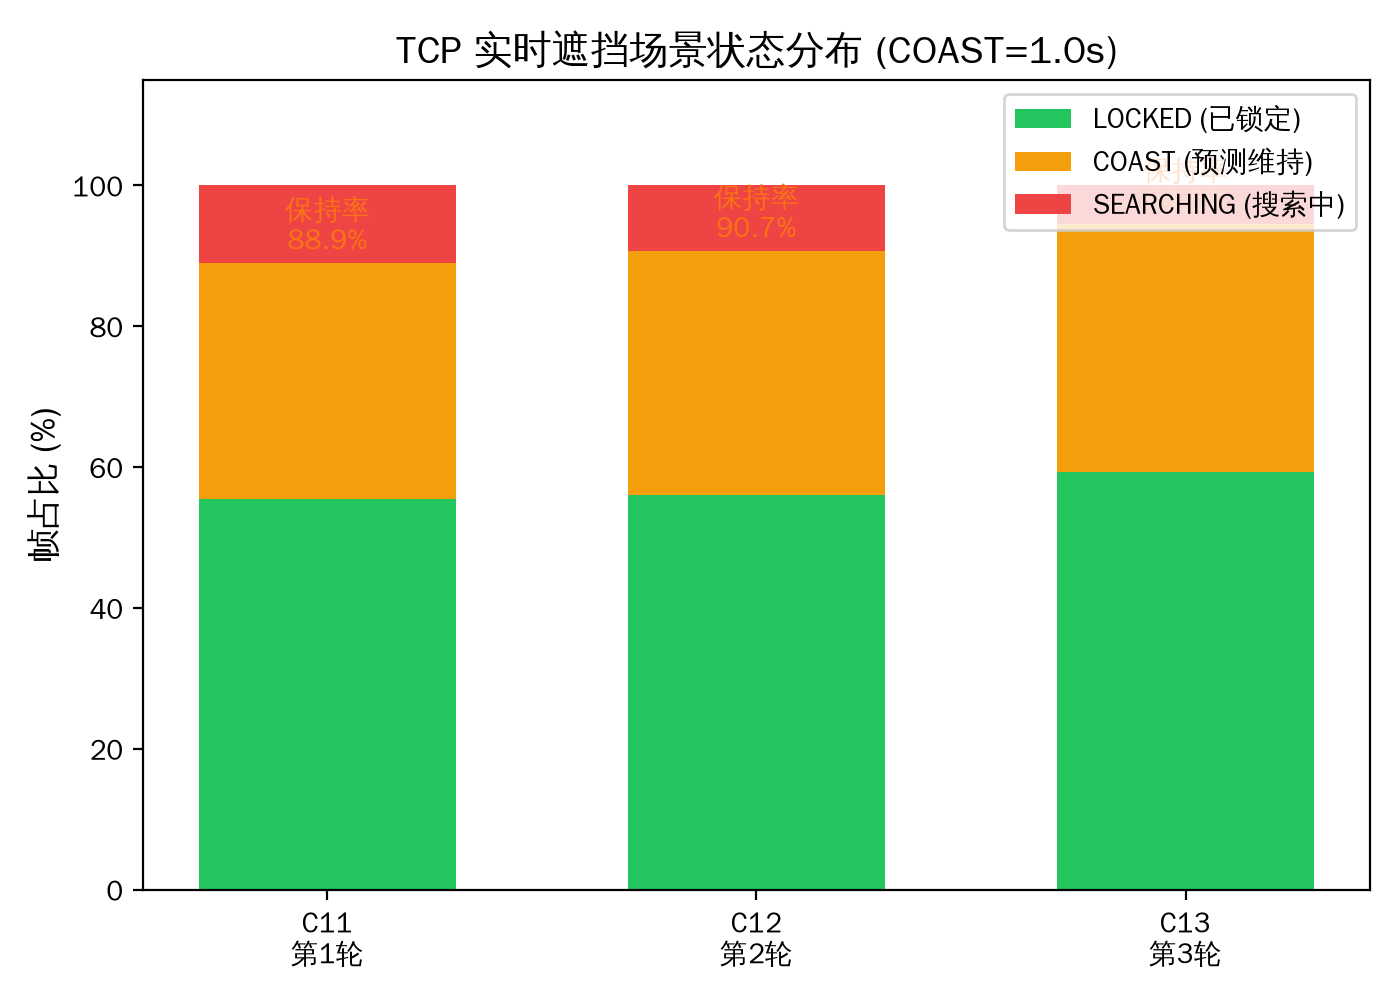
\includegraphics[width=0.72\textwidth]{images/pictures/chart_tcp_state.png}
\caption{TCP 遮挡用例的状态时序与持续时间分布}
\label{fig:coast_timeline}
\end{figure}

\subsection{真实场景录像}

在真实场景录像（C04）中，目标频繁进出树丛，锁定率仅 23.2\%，但航迹保持率达到 99.3\%。这一结果看似矛盾，实则说明：绝大多数帧虽然没有检测，但目标并未真正丢失，COAST 能够持续维持航迹；只有在目标真正飞出视场或长时间被遮挡时，系统才回到 SEARCH。这验证了"锁定率低不等于系统失效"的判断，也说明在评估跟踪系统时，航迹保持率比单帧锁定率更能反映实际可用性。

\section{设计讨论}

\subsection{为什么不用多目标跟踪框架}

SORT\cite{sort} 与 DeepSORT\cite{deepsort} 等框架面向多目标场景，包含轨迹管理、外观特征提取与匈牙利匹配等组件。本文的系统面向单目标反无人机场景，同一时刻只需要跟踪一个最具威胁的目标，因此不需要复杂的轨迹管理。简化的状态机具有三点优势：计算开销极低、行为可解释、参数易于现场调整。若未来需要同时跟踪多架无人机，可以在状态机之上增加轨迹池与数据关联层，而不需要推翻现有设计。

\subsection{为什么用状态机而不是有限状态自动机的形式化方法}

本文的状态机在形式上是一个确定性有限状态自动机，但本文没有采用模型检验等形式化方法，原因是：系统的输入是连续的视频流，状态转移依赖置信度、距离等连续量，形式化建模的收益有限；工程上更重要的是参数可调、日志可追溯。本文通过 14 个用例的回归测试来保证行为正确，而不是通过形式化证明。

\subsection{失效边界}

状态机的有效性依赖两个假设：目标在相邻帧间的位移不超过空间门限；遮挡时间不超过 COAST 时限。当目标以极高速度飞行（例如穿越机以 30\,m/s 飞行）或长时间被完全遮挡（例如穿过多层建筑）时，系统会丢失目标。这是设计上的取舍，本文在第九章的"能力边界"一节中如实讨论。

\section{本章小结}

本章针对检测输出直接使用导致的误检、跳变与遮挡问题，设计了 SEARCH/LOCKED/COAST 三态跟踪状态机。SEARCH 采用 0.25/0.55 双门限与空域先验，防止误锁；LOCKED 采用 140\,px 空间门限的最近邻关联与三维量测卡尔曼滤波，防止跳变并平滑输出；COAST 采用 1.0\,s 预测维持，防止短时遮挡中断。参数选择均有明确的物理依据，算法复杂度为 $O(N)$，对系统实时性无影响。实验表明，遮挡场景的航迹保持率达到 88.9\%--94.5\%，真实场景录像达到 99.3\%，验证了状态机的有效性。
